% Options for packages loaded elsewhere
\PassOptionsToPackage{unicode}{hyperref}
\PassOptionsToPackage{hyphens}{url}
%
\documentclass[
  ignorenonframetext,
]{beamer}
\usepackage{pgfpages}
\setbeamertemplate{caption}[numbered]
\setbeamertemplate{caption label separator}{: }
\setbeamercolor{caption name}{fg=normal text.fg}
\beamertemplatenavigationsymbolsempty
% Prevent slide breaks in the middle of a paragraph
\widowpenalties 1 10000
\raggedbottom
\setbeamertemplate{part page}{
  \centering
  \begin{beamercolorbox}[sep=16pt,center]{part title}
    \usebeamerfont{part title}\insertpart\par
  \end{beamercolorbox}
}
\setbeamertemplate{section page}{
  \centering
  \begin{beamercolorbox}[sep=12pt,center]{part title}
    \usebeamerfont{section title}\insertsection\par
  \end{beamercolorbox}
}
\setbeamertemplate{subsection page}{
  \centering
  \begin{beamercolorbox}[sep=8pt,center]{part title}
    \usebeamerfont{subsection title}\insertsubsection\par
  \end{beamercolorbox}
}
\AtBeginPart{
  \frame{\partpage}
}
\AtBeginSection{
  \ifbibliography
  \else
    \frame{\sectionpage}
  \fi
}
\AtBeginSubsection{
  \frame{\subsectionpage}
}
\usepackage{amsmath,amssymb}
\usepackage{lmodern}
\usepackage{ifxetex,ifluatex}
\ifnum 0\ifxetex 1\fi\ifluatex 1\fi=0 % if pdftex
  \usepackage[T1]{fontenc}
  \usepackage[utf8]{inputenc}
  \usepackage{textcomp} % provide euro and other symbols
\else % if luatex or xetex
  \usepackage{unicode-math}
  \defaultfontfeatures{Scale=MatchLowercase}
  \defaultfontfeatures[\rmfamily]{Ligatures=TeX,Scale=1}
  \setmainfont[BoldFont = SF Pro Rounded Semibold]{SF Pro Rounded}
  \setmathfont[]{STIX Two Math}
\fi
\usefonttheme{serif} % use mainfont rather than sansfont for slide text
% Use upquote if available, for straight quotes in verbatim environments
\IfFileExists{upquote.sty}{\usepackage{upquote}}{}
\IfFileExists{microtype.sty}{% use microtype if available
  \usepackage[]{microtype}
  \UseMicrotypeSet[protrusion]{basicmath} % disable protrusion for tt fonts
}{}
\makeatletter
\@ifundefined{KOMAClassName}{% if non-KOMA class
  \IfFileExists{parskip.sty}{%
    \usepackage{parskip}
  }{% else
    \setlength{\parindent}{0pt}
    \setlength{\parskip}{6pt plus 2pt minus 1pt}}
}{% if KOMA class
  \KOMAoptions{parskip=half}}
\makeatother
\usepackage{xcolor}
\IfFileExists{xurl.sty}{\usepackage{xurl}}{} % add URL line breaks if available
\IfFileExists{bookmark.sty}{\usepackage{bookmark}}{\usepackage{hyperref}}
\hypersetup{
  pdftitle={305 Lecture 10.1 - Learning from Evidence},
  pdfauthor={Brian Weatherson},
  hidelinks,
  pdfcreator={LaTeX via pandoc}}
\urlstyle{same} % disable monospaced font for URLs
\newif\ifbibliography
\usepackage{graphicx}
\makeatletter
\def\maxwidth{\ifdim\Gin@nat@width>\linewidth\linewidth\else\Gin@nat@width\fi}
\def\maxheight{\ifdim\Gin@nat@height>\textheight\textheight\else\Gin@nat@height\fi}
\makeatother
% Scale images if necessary, so that they will not overflow the page
% margins by default, and it is still possible to overwrite the defaults
% using explicit options in \includegraphics[width, height, ...]{}
\setkeys{Gin}{width=\maxwidth,height=\maxheight,keepaspectratio}
% Set default figure placement to htbp
\makeatletter
\def\fps@figure{htbp}
\makeatother
\setlength{\emergencystretch}{3em} % prevent overfull lines
\providecommand{\tightlist}{%
  \setlength{\itemsep}{0pt}\setlength{\parskip}{0pt}}
\setcounter{secnumdepth}{-\maxdimen} % remove section numbering
\let\Tiny=\tiny

 \setbeamertemplate{navigation symbols}{} 

% \usetheme{Madrid}
 \usetheme[numbering=none, progressbar=foot]{metropolis}
 \usecolortheme{wolverine}
 \usepackage{color}
 \usepackage{MnSymbol}
% \usepackage{movie15}

\usepackage{amssymb}% http://ctan.org/pkg/amssymb
\usepackage{pifont}% http://ctan.org/pkg/pifont
\newcommand{\cmark}{\ding{51}}%
\newcommand{\xmark}{\ding{55}}%

\DeclareSymbolFont{symbolsC}{U}{txsyc}{m}{n}
\DeclareMathSymbol{\boxright}{\mathrel}{symbolsC}{128}
\DeclareMathAlphabet{\mathpzc}{OT1}{pzc}{m}{it}

 \usepackage{tikz-qtree}
% \usepackage{markdown}
%\RequirePackage{bussproofs}
\RequirePackage[tableaux]{prooftrees}
\usetikzlibrary{arrows.meta}
 \forestset{line numbering, close with = x}
% Allow for easy commas inside trees
\renewcommand{\,}{\text{, }}


\usepackage{tabulary}

\usepackage{open-logic-config}

\setlength{\parskip}{1ex plus 0.5ex minus 0.2ex}

\AtBeginSection[]
{
\begin{frame}
	\Huge{\color{darkblue} \insertsection}
\end{frame}
}

\renewenvironment*{quote}	
	{\list{}{\rightmargin   \leftmargin} \item } 	
	{\endlist }

\definecolor{darkgreen}{rgb}{0,0.7,0}
\definecolor{darkblue}{rgb}{0,0,0.8}

\newcommand{\starttab}{\begin{center}
\vspace{6pt}
\begin{tabular}}

\newcommand{\stoptab}{\end{tabular}
\vspace{6pt}
\end{center}
\noindent}


\newcommand{\sif}{\rightarrow}
\newcommand{\siff}{\leftrightarrow}
\newcommand{\EF}{\end{frame}}


\newcommand{\TreeStart}[1]{
%\end{frame}
\begin{frame}
\begin{center}
\begin{tikzpicture}[scale=#1]
\tikzset{every tree node/.style={align=center,anchor=north}}
%\Tree
}

\newcommand{\TreeEnd}{
\end{tikzpicture}
%\end{center}
}

\newcommand{\DisplayArg}[2]{
\begin{enumerate}
{#1}
\end{enumerate}
\vspace{-6pt}
\hrulefill

%\hspace{14pt} #2
%{\addtolength{\leftskip}{14pt} #2}
\begin{quote}
{\normalfont #2}
\end{quote}
\vspace{12pt}
}

\newenvironment{ProofTree}[1][1]{
\begin{center}
\begin{tikzpicture}[scale=#1]
\tikzset{every tree node/.style={align=center,anchor=south}}
}
{
\end{tikzpicture}
\end{center}
}

\newcommand{\TreeFrame}[2]{
\begin{columns}[c]
\column{0.5\textwidth}
\begin{center}
\begin{prooftree}{}
#1
\end{prooftree}
\end{center}
\column{0.45\textwidth}
%\begin{markdown}
#2
%\end{markdown}
\end{columns}
}

\newcommand{\ScaledTreeFrame}[3]{
\begin{columns}[c]
\column{0.5\textwidth}
\begin{center}
\scalebox{#1}{
\begin{prooftree}{}
#2
\end{prooftree}
}
\end{center}
\column{0.45\textwidth}
%\begin{markdown}
#3
%\end{markdown}
\end{columns}
}

\usepackage[bb=boondox]{mathalfa}
\DeclareMathAlphabet{\mathbx}{U}{BOONDOX-ds}{m}{n}
\SetMathAlphabet{\mathbx}{bold}{U}{BOONDOX-ds}{b}{n}
\DeclareMathAlphabet{\mathbbx} {U}{BOONDOX-ds}{b}{n}


\newenvironment{oltableau}{\center\tableau{}} %wff format={anchor = base west}}}
       {\endtableau\endcenter}
       
\newcommand{\formula}[1]{$#1$}

\usepackage{tabulary}
\usepackage{booktabs}

\def\begincols{\begin{columns}}
\def\begincol{\begin{column}}
\def\endcol{\end{column}}
\def\endcols{\end{columns}}

\usepackage[italic]{mathastext}
\usepackage{nicefrac}

\definecolor{mygreen}{RGB}{0, 100, 0}
\definecolor{mypink2}{RGB}{219, 48, 122}
\definecolor{dodgerblue}{RGB}{30,144,255}

%\def\True{\textcolor{dodgerblue}{\text{T}}}
%\def\False{\textcolor{red}{\text{F}}}

\def\True{\mathbb{T}}
\def\False{\mathbb{F}}

% This is because arguments didn't have enough space after them
\usepackage{etoolbox}
\AfterEndEnvironment{description}{\vspace{9pt}}
\AfterEndEnvironment{oltableau}{\vspace{9pt}}
\BeforeBeginEnvironment{oltableau}{\vspace{9pt}}
\AfterEndEnvironment{center}{\vspace{12pt}}
\BeforeBeginEnvironment{tabular}{\vspace{9pt}}

\setlength\heavyrulewidth{0pt}
\setlength\lightrulewidth{0pt}

%\def\toprule{}
%\def\bottomrule{}
%\def\midrule{}

\setbeamertemplate{caption}{\raggedright\insertcaption}

\ifluatex
  \usepackage{selnolig}  % disable illegal ligatures
\fi

\title{305 Lecture 10.1 - Learning from Evidence}
\author{Brian Weatherson}
\date{}

\begin{document}
\frame{\titlepage}

\begin{frame}{Plan}
\protect\hypertarget{plan}{}
\begin{itemize}
\tightlist
\item
  Today we're going to talk a bit about how to learn from uncertain
  data.
\item
  We've talked a bit about the mathematics of how to update in clear
  cases.
\item
  Today we're going to talk about less clear cases.
\item
  And to do that, it helps to start with a story.
\end{itemize}
\end{frame}

\begin{frame}{Associated Reading}
\protect\hypertarget{associated-reading}{}
\begin{itemize}
\tightlist
\item
  This is a build up to part 3 of Odds and Ends, but this particular
  story isn't in the book.
\item
  It's too good a story to leave out though.
\end{itemize}
\end{frame}

\begin{frame}{Abraham Wald}
\protect\hypertarget{abraham-wald}{}
\begin{columns}[c]
\begin{column}{0.48\textwidth}
\begin{figure}
\centering
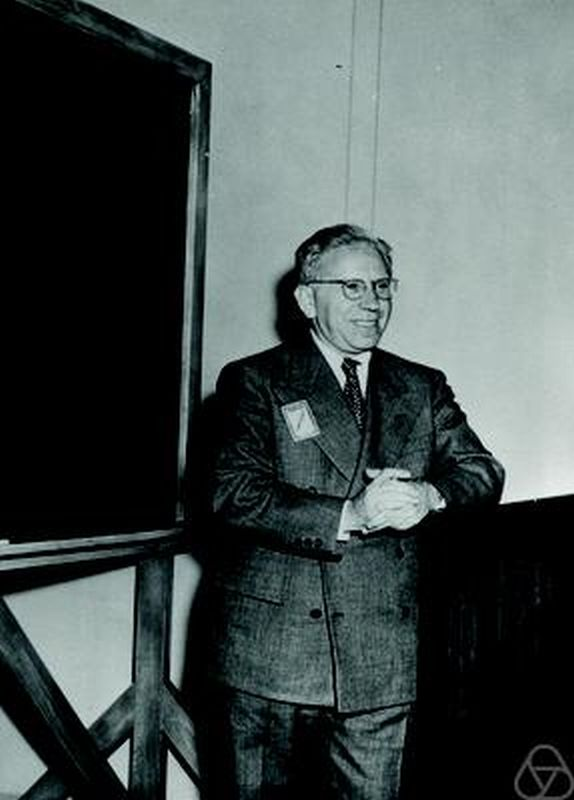
\includegraphics{../images/week10/wald_photo.jpg}
\caption{Abraham Wald}
\end{figure}
\end{column}

\begin{column}{0.48\textwidth}
We're going to do a bit of math, but we'll start with a point made by
someone who was a mathematician (and a good one) that doesn't require
any math.
\end{column}
\end{columns}
\end{frame}

\begin{frame}{Surviving Gunfire}
\protect\hypertarget{surviving-gunfire}{}
\begin{itemize}
\tightlist
\item
  The backstory is that during WWII the Allies were losing a lot of
  planes to German artillery.
\item
  They were thinking about how to add armor to the planes in order to
  defend them better.
\item
  So they investigated the planes that had come back to see where they
  were getting most bullet holes, and planned to add extra armor to
  those parts.
\end{itemize}
\end{frame}

\begin{frame}{The Evidence}
\protect\hypertarget{the-evidence}{}
\begin{columns}[c]
\begin{column}{0.48\textwidth}
\begin{figure}
\centering
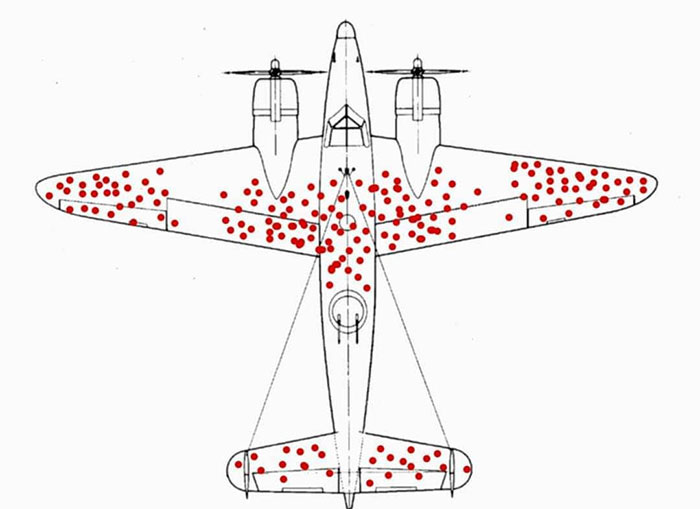
\includegraphics{../images/week10/wald_plane.jpg}
\caption{Bulletholes}
\end{figure}
\end{column}

\begin{column}{0.48\textwidth}
Here's a representation of where they found holes in the planes.
\end{column}
\end{columns}
\end{frame}

\begin{frame}{Policy}
\protect\hypertarget{policy}{}
\begin{columns}[c]
\begin{column}{0.48\textwidth}
\begin{figure}
\centering
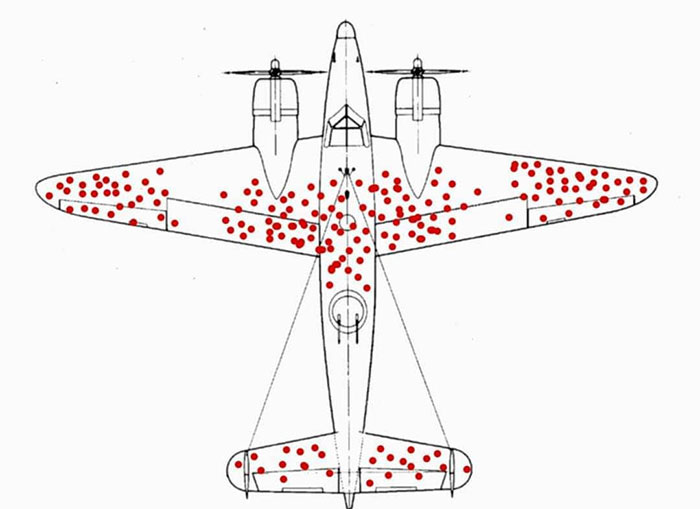
\includegraphics{../images/week10/wald_plane.jpg}
\caption{Bulletholes}
\end{figure}
\end{column}

\begin{column}{0.48\textwidth}
Where should they add the armor?
\end{column}
\end{columns}
\end{frame}

\begin{frame}{Wald's Answer}
\protect\hypertarget{walds-answer}{}
\begin{columns}[c]
\begin{column}{0.48\textwidth}
\begin{figure}
\centering
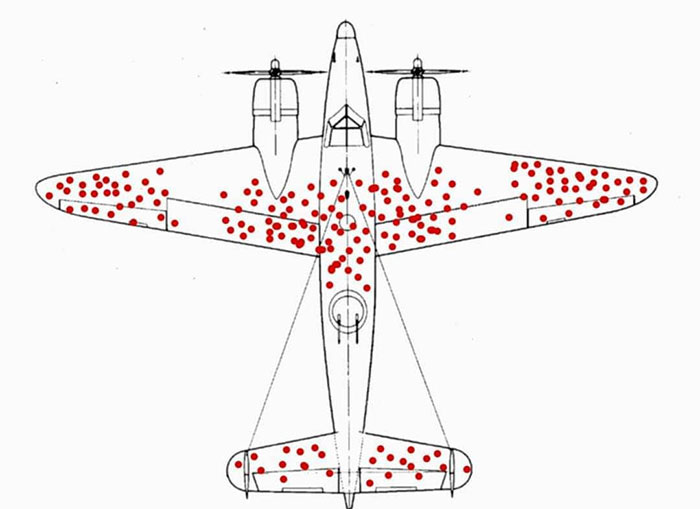
\includegraphics{../images/week10/wald_plane.jpg}
\caption{Bulletholes}
\end{figure}
\end{column}

\begin{column}{0.48\textwidth}
You should put the extra armor where the holes aren't.
\end{column}
\end{columns}
\end{frame}

\begin{frame}{Hypothesis One - The Original Airforce View}
\protect\hypertarget{hypothesis-one---the-original-airforce-view}{}
\begin{itemize}
\tightlist
\item
  The planes coming back are our best sample of the planes in the field.
\item
  The bullet holes in them are asymmetrically distributed.
\item
  So that's evidence that certain parts of the planes are more likely to
  get hit.
\item
  And that's where we should add extra protection.
\end{itemize}
\end{frame}

\begin{frame}{Hypothesis Two - Wald's View}
\protect\hypertarget{hypothesis-two---walds-view}{}
\begin{itemize}
\tightlist
\item
  Bullet holes are almost surely randomly distributed.
\item
  The planes coming back are not a random sample of the planes in the
  air.
\item
  They do not include all of the planes that crashed.
\item
  The best explanation of the asymmetry is that the `missing' bullet
  holes are for the planes that crashed.
\item
  And the best explantion in turn for that is that those are the places
  where bullet holes are fatal to the plane.
\end{itemize}
\end{frame}

\begin{frame}{Who Was Right}
\protect\hypertarget{who-was-right}{}
\begin{itemize}
\tightlist
\item
  We nowadays think Wald was.
\item
  Artillery, especially artillery of that era, is really a random
  process.
\item
  Moreover, the places with no holes - the engines and the cockpit - are
  just where you'd expect fatal injuries to occur.
\item
  So the thing to do was to protect those areas, and try to turn fatal
  injuries into non-fatal ones.
\end{itemize}
\end{frame}

\begin{frame}{Big Lesson}
\protect\hypertarget{big-lesson}{}
When you see that \(p\) is true, there are two different possible
lessons to learn.

\begin{enumerate}
\tightlist
\item
  \(p\) is true.
\item
  I'm seeing that \(p\) is true.
\end{enumerate}

Very often, the second is the right lesson to draw.
\end{frame}

\begin{frame}{Example}
\protect\hypertarget{example}{}
\begin{columns}[c]
\begin{column}{0.48\textwidth}
\begin{figure}
\centering
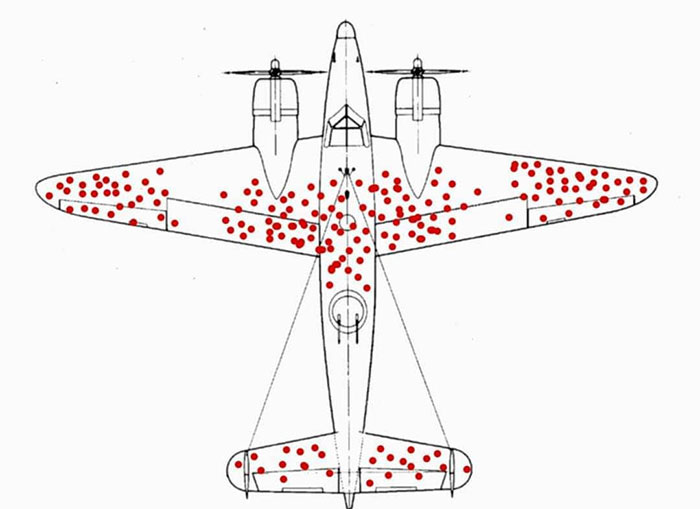
\includegraphics{../images/week10/wald_plane.jpg}
\caption{Bulletholes}
\end{figure}
\end{column}

\begin{column}{0.48\textwidth}
\begin{itemize}
\tightlist
\item
  A plane comes back with a bullethole in its left wing.
\item
  That tells us that this plane got shot in the left wing.
\item
  It also tells us, from the fact that we can see that this plane got
  shot in the left wing, that this damage is non-fatal.
\end{itemize}
\end{column}
\end{columns}
\end{frame}

\begin{frame}{Big Picture}
\protect\hypertarget{big-picture}{}
\begin{itemize}
\tightlist
\item
  We want to learn from our evidence.
\item
  But sometimes that requires thinking about why we got just this
  evidence.
\item
  And to do that it helps to have a theory about how to think about how
  evidence bears on uncertainty.
\end{itemize}
\end{frame}

\begin{frame}{For Next Time}
\protect\hypertarget{for-next-time}{}
We'll talk about an error in thinking probabilistically that some people
make - the gambler's fallacy.
\end{frame}

\end{document}
